\documentclass[conference]{IEEEtran}
\IEEEoverridecommandlockouts
% The preceding line is only needed to identify funding in the first footnote. If that is unneeded, please comment it out.
\usepackage{cite}
\usepackage{amsmath,amssymb,amsfonts}
\usepackage{algorithmic}
\usepackage{graphicx}
\usepackage{textcomp}
\usepackage{xcolor}

\usepackage{url}
\def\UrlFont{\rmfamily}
\usepackage{graphicx}

\usepackage{graphicx}
\usepackage{caption}
\usepackage{subfigure}
\usepackage{float}
\usepackage{amsmath}
\usepackage{amssymb}
\usepackage{multirow}
\usepackage{tabularx} 
\usepackage{array} 
\usepackage{booktabs} 
\usepackage{setspace}
\usepackage{url}
\usepackage[ hyperfootnotes=true, colorlinks=true, linkcolor=blue,urlcolor=blue,filecolor=blue, citecolor=cyan, anchorcolor=blue]{hyperref}




\def\BibTeX{{\rm B\kern-.05em{\sc i\kern-.025em b}\kern-.08em
    T\kern-.1667em\lower.7ex\hbox{E}\kern-.125emX}}
\begin{document}

\title{BASD-SLAM: A Deep-Learning Visual SLAM System Based On Binary Adaptive-Scale descriptor}

\author{\IEEEauthorblockN{1\textsuperscript{st} Given Name Surname}
\IEEEauthorblockA{\textit{dept. name of organization (of Aff.)} \\
\textit{name of organization (of Aff.)}\\
City, Country \\
email address or ORCID}
\and
\IEEEauthorblockN{2\textsuperscript{nd} Given Name Surname}
\IEEEauthorblockA{\textit{dept. name of organization (of Aff.)} \\
\textit{name of organization (of Aff.)}\\
City, Country \\
email address or ORCID}
\and
\IEEEauthorblockN{3\textsuperscript{rd} Given Name Surname}
\IEEEauthorblockA{\textit{dept. name of organization (of Aff.)} \\
\textit{name of organization (of Aff.)}\\
City, Country \\
email address or ORCID}
\and
\IEEEauthorblockN{4\textsuperscript{th} Given Name Surname}
\IEEEauthorblockA{\textit{dept. name of organization (of Aff.)} \\
\textit{name of organization (of Aff.)}\\
City, Country \\
email address or ORCID}
\and
\IEEEauthorblockN{5\textsuperscript{th} Given Name Surname}
\IEEEauthorblockA{\textit{dept. name of organization (of Aff.)} \\
\textit{name of organization (of Aff.)}\\
City, Country \\
email address or ORCID}
\and
\IEEEauthorblockN{6\textsuperscript{th} Given Name Surname}
\IEEEauthorblockA{\textit{dept. name of organization (of Aff.)} \\
\textit{name of organization (of Aff.)}\\
City, Country \\
email address or ORCID}
}

\maketitle









%%%%%%%%%%%%%%%%%%%%%%%
\begin{abstract}
The feature quality plays an important role in visual SLAM (Visual Simultaneous Localization and Mapping) based on feature descriptor matching, and becomes the bottleneck of positioning accuracy improvement. Now lots of hand-crafted descriptors like BRIEF and ORB don't work very well in complex scenarios. The Convolutional Neural Network is proved to have tremendous advantages on image feature extraction. In this paper, we design a CNN model to extract binary visual feature descriptor from image patches. Based on this deep feature descriptor, we design a monocular SLAM system, named BASD-SLAM, by replacing ORB descriptor in ORB-SLAM2. We also train visual Bag of Words to detect loop closure. Experiments show that our BASD achieves better results on the HPatches dataset and UBC benchmark. In the meantime, the BASD-SLAM system outperforms other current popular SLAM system on Tartanair dataset.
%%%%%%%%%%%%%%%%%%%%%%%%%%%%%%%%%%%%%%%%%%%%%%%%

% We would like to encourage you to list your keywords within
% the abstract section using the \keywords{...} command.

\end{abstract}

\begin{IEEEkeywords}
binary descriptor,deep learning,SLAM
\end{IEEEkeywords}
%%%%%%%%%%%%%%%%%%%%%%%%%%%%%%%%%%%%%%%%%%%%%%%%%%%%%%%%%%%%%%%%%%%%%%%%%%%%%%%%%%%%%%%%%%%%%%%%%%%%


%%%%%%%%%%%%%%%%%%%%%%%%%%%%%%%%%%%%%%%%%%%%%%%%%%%%%%%%%%%%%%%%%%%%%%%%%%%%%%%%


%%%%%%%%%%%%%%%%%%%%%%%%%%%%%%%%%%%%%%%%%%%%%%%%%%%%%%%%%%%%%%%%%%%%%%%%%%%%%%%%
\section{INTRODUCTION}

Visual SLAM has got prosperous development in recent years. The result of feature matching in the keypoint-based vSLAM system depends on the local descriptor quality. The traditional descriptors rely on the pixel-level match,and the match error will accumulate slowly, finally impact the pose estimation result. So improving the descriptor quality is of high significance.

With the fast development of deep learning in recent years,  image proccessing based on DL has become more and more popular. And vast researches have proved the unparalleled advantages on image feature extraction and data association, which are the bottleneck of traditonal visual SLAM pipeline. As a result, lots of researchers are committed to apply deep learining to SLAM,and solve the bottleneck problems,like feature extraction and data association.

There have tremendous researches indicate the application of deep learining in SLAM improving the accuracy of vSLAM. Many researchers take advantage of deep learing ,and substitute some modules in the traditional SLAM pipeline, such as feature matching, relocalization, and so on. Some also use high-level semantic information, which can help the SLAM relocalization, bundle adjustment, etc. And some end-to-end SLAM system  ,which generates pose estimation directly from pictures ,also achieve better results in specific scenarios.

However, there are many problems on the application of deep learning in SLAM system. For example, end-to-end SLAM systems are dependent on specific scenarios, and generalization ability are not strong.Semantic SLAM cannot guarantee the  appearance of specific semantic information,like the chairs in SLAM++; While the extraction of low-level features does not take into account the scale problem[ASD-SLAM],which makes the descriptors such as hardnet not suitable for SLAM.

To address the limitation of above researches, we propose our local feature descriptor extraction neural network, whcih address the scale problem causing deep descriptor aren't suitable for SLAM. the propoesed descriptor shares same structure with ORB, so it can be  easyily implemented on popular SLAM framework.To achieve better efficiency, we binarize our descriptor,which can vastly speed up the descriptor matching process.We also train Bag-of-Words for our deep descriptor to realize loop closure. 

In addition, our descriptor can also be extended to other similar fields like SFM. In summary, our main contributions are the following:
\begin{itemize}
\item We propose a binary descriptor with CNN model using four loss function, and outperforms other traditional descriptor on accuracy and effectiveness. 
\item We design a monocular system with our learned descriptor, and achieve better results than other traditional visual SLAM system on several benchmark datasets.
\end{itemize}

%%%%%%%%%%%%%%%%%%%%%%%%%%%%%%%%%%%%%%%%%%%%%%%%%%%%%%%%%%%%%%%%%%%%%%%%%%%%%%%%%
\section{RELATED WORK}
Since this paper is aimming at learning suitable local descriptor which can enhance visual SLAM system, in this section we review related works with respect to the two fields that we integrate within our research, local feature descriptor learning and deep learning enhanced SLAM.

\subsection{Local Feature Descriptor}
With the progress of feature matching,many local features have been proposed. 
SIFT\cite{c6} can be invirant to image scaling,rotation,and even affine transformation. this descriptor performes stablly well, but needs considerably lots of computating power. 
BRIEF\cite{c7} chose $n_{d}$ pixel pairs in some specific sampling ways in smoothed image patch, and calculated binary descriptor by comparing gray values between pixel pairs. It accelerated feature descriptor extraction,but was very sensitive to patch rotation.  
Based on BRIEF, ORB\cite{c8} achieved rotation inviariance by calculating principal direction of image patches,and rotating image patches to same direction. ORB also was inviariant to scale change by image pyramid application.
There also exsited many learned descriptors based on these traditional descriptor like PCA-SIFT\cite{c9},BinBoost\cite{c10}, RMGD\cite{c11} ,etc,which improve the real-time performance by mapping high-dimensional space to low-dimensional space. 

In recent years,deep learning shines in image process,so many researches apply Deep learning to descriptor generation ,and these learning descriptor are more robust to transformations like illumination or viewpoint change .In order to pursue the accuracy and robustness of image matching, many researches proposed float deep learning local descriptor.
[SuperPoint]\cite{c12} presented and end-to-end fully-convolutional network to jointly detect interesting point and  generate descriptor on full-sized images according to Homographic Adaptation on the dataset.
[MatchNet]\cite{c13} utilized  siamese network to extract feature descriptor and processed metric learning followed by a fully-connected network.
[L2-Net]\cite{c14} proposed a leadrning descriptor which could be matched through $L_{2}$ distance ,genrated by a CNN model without metric learning layer. They used a novel sampling strategy to obtain much more training samples in few training epochs.
[HardNet] \cite{c15} presented a metirc learning loss,which maximized the distance between positive and negative example in one batch.This method worked very well in shallow network structure,which showed the advantage on complex regularization method.

In order to compensate for the slow matching speed and large calculation cost of float learning descriptor, many researches are devoted to exploring the binarization method of float descriptor.
	[Deep  multi-quantization network]\cite{c16} utilized K-Autoencoders baed on metric learning to realize binarization,which jointly optimized the parameters of feature extraction and  binarization.But the deep network structure  decided  real-time performance not very good. 
[Learning to Hash  with DBNN]\cite{c17} proposed a supervised and unsupervised binarization hashing deep learning model,which consited of a hidden layer to directly output binarization codes. This method abandoned sign or step function to binarize descriptor, but caused the training process much more complex. 
[CDBin]\cite{c18} just added sign function in the loss function to realize binarization, which was very direct and efficient.

\subsection{Deep learning enhanced SLAM}
Deep learning is a powerful method to solve feature extraction and data association problems encountered in the traditional SLAM framework. 
DeepVO \cite{c19}abandoned traditional SLAM pipeline, and proposed a novel compact end-to-end SLAM system using recurrent convolutional neural networks,which could directly infer camera poses from raw RGB images(videos) .They firstly adopted RNNs to model sequential learning,and achieved better results on KITTI datasets. 
[Unsupervised Learning of Depth and Ego-Motion from Video]\cite{c20} explored an unsupervised learning framework,which consisted of two CNNs to infer depth and pose respectively, to estimate monocular depth and camera motion simultaneously. They just used video data to train their network,which can be helpful to network training.
[DeMoN]\cite{c21} proposed multiple encoder-decoder convolutional neural networks to estimate depth and ego-motion from two successive images.It learned matching concept from training.Althought end-to-end SLAM makes SLAM system more compact, it lacks of model generalization ability.

End-to-end SLAM doesn't show advantages on traditional SLAM pipeline because it lacks of clear reasearch model support. Intead of traditional local descriptor, many researches are devoted to apply high-level semantic information to improve SLAM performace. 
SLAM++ \cite{c22}ultilized repeated objects and special structures to construct object graph, and perform ICP to estimate camera pose.  
[Long-term Visual Localization using Semantically Segmented Images] \cite{c23}relocalized with semantically segmented objects based on particle filter. Instead of traditional local features,they could realize long-term localization with image segmenter. Because segmenting error, they only realized meter-level positioning.  
[View-Invariant Loop Closure with Oriented Semantic Landmarks] \cite{c24}proposed semantic monocular SLAM system  to utilize object geometry for loop-closure detection in big perspective change.their novel object orientation estimation method  leveraged object tracking accuracy in the ambiguous situation caused by object symmetry.



%%%%%%%%%%%%%%%%%%%%%%%%%%%%%%%%%%%%%%%%%%%%%%%%%%%%%%%%%%%%%%%%%%%%%%%%%%%%%%%%%
\section{System Overview}
In our BASD-SLAM system, we still adopt traditional visual SLAM pipeline. ORB-SLAM2 \cite{c25}is a classical visual SLAM system. Unlike other end-to-end SLAM system, we just replace the traditional hand-crafted descriptor ORB with our learned descriptor and evaluate the efficiency and effectiveness of our descriptor. This also enables our descriptor suitable to other SLAM system like SFM.


\begin{figure}[h]
\centering
%三个结果应该上下排列
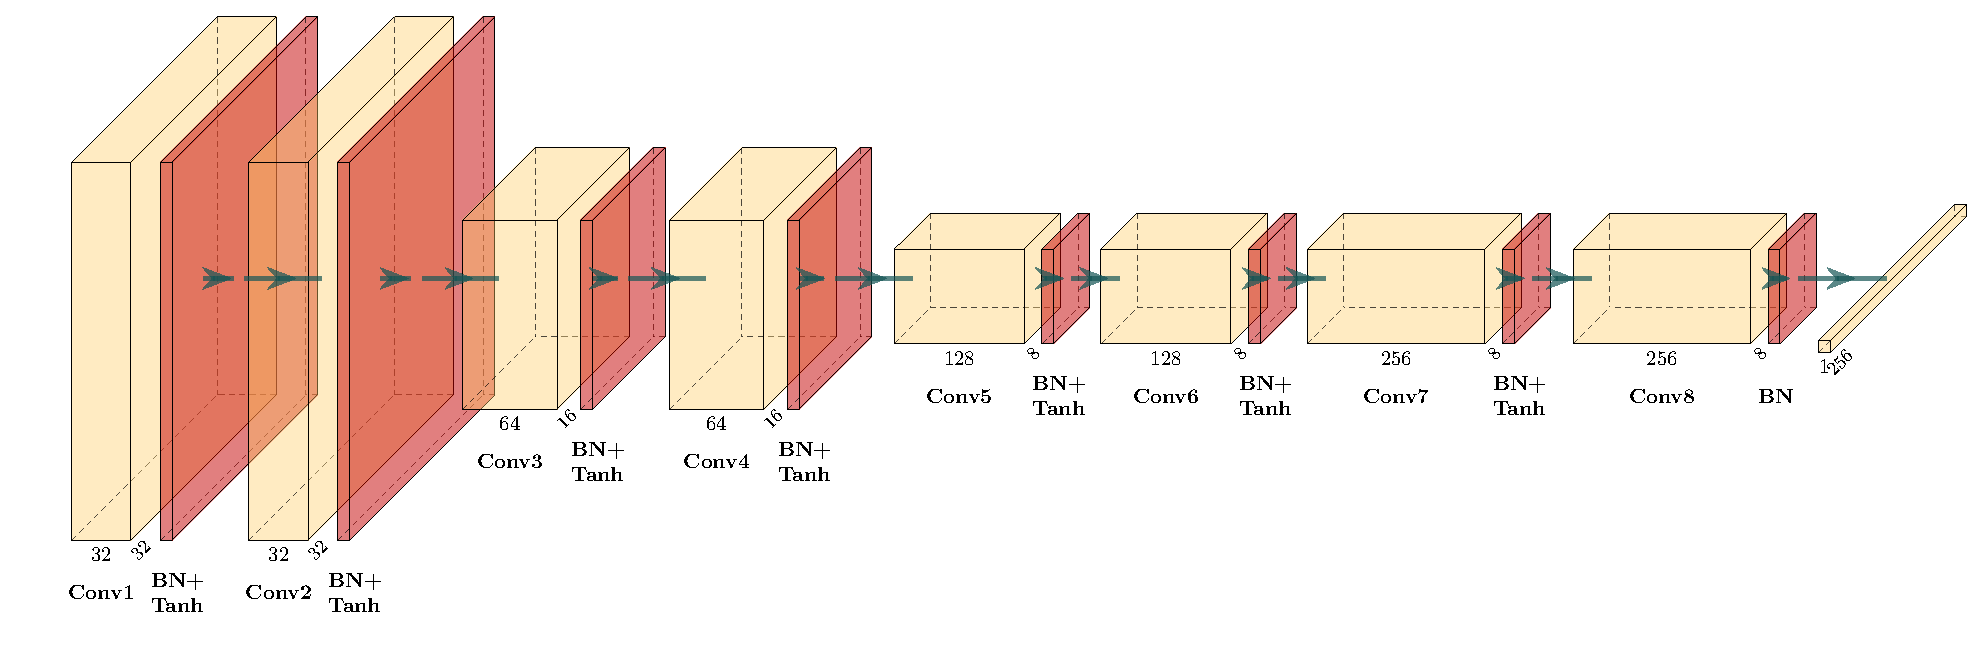
\includegraphics[scale=0.36]{BASD_Net}
\captionsetup{font={scriptsize}}
\caption{ illustration of our learning binary local descriptor architecture.} \scriptsize
\end{figure}

\subsection{Local feature design } 
Compared with hand-crafted methods, learned descriptors has tremendous advantages, such as compact structure, evenly distribution, robust to noise and so on. Moreover, learning-based descriptors are data-adaptive. In order to make our descriptor more effective, we just adopt shallow convolutional neural network to generate our descriptor, and the shallow network has also been proved to be suitable to extract low-level image information [14]. float descriptors sacrifice the effectiveness of feature matching and loop closure. Instead, our shallow network will obtain binary local feature descriptor, and also maintain the high precision.
	[15] reveals that triplet network has greater advantages in metric learning than Siamese network, so we also adopt the former to train our descriptor. There are eight convolutional layers, each of which is followed by a Tanh non-linearity and Batch Norm operations. And the output of network is normalized to unit-length. In order to reduce the possibility of overfitting, we add a dropout layer in the last of our network. After lots of tuning step and training process, we set the dropout rate to 0.3.
	Loss function plays an important role in descriptor generation. We adopt four loss type to train our descriptor. We will describe in detail below.

\subsubsection{Adaptive-Scale Triplet Loss} 
Triplet loss has been proved to have great advantages in descriptor generation. So we also adopt this loss function. \cite{c28}proposed the scale uncertainty influence in triplet loss, and modified the prime triplet loss function to reflect the changes of scale by adding a scale reminder factor. Given three image patches, Pa, Pb and Pc, which represent the anchor, positive and negative image patches. After the reasoning of network, we get descriptors xa, xb and xc respectively. And the adaptive-scale triplet loss function is defined as:

\begin{equation}
d _{+} = \| x_{a} - x_{p}  \| 
\end{equation}

\begin{equation}
d _{-} = \| x_{a} - x_{n}  \| 
\end{equation}

\begin{equation}
\xi  = \frac{d _{-}}{d _{+}}
\end{equation}

\begin{equation}
L_{trip}  = - \frac{1}{\xi}\log (smax(\xi( d _{-} - d _{+}  ) , 0)) 
\end{equation}

Where d- and d+ is the L2 distance of anchor descriptor with negative descriptor, anchor descriptor with positive descriptor, respectively. 

Because we set batch size to 1024, so the choice of d- and d+ matters. We also adopt the adaptive-scale sampling strategy to obtain suitable d- and d+.

The native training strategy is too complex and performs not well, so we turn to the hard negative mining strategy proposed in \cite{c15}, which is proved to be effective and easy to converge in training. 

\subsubsection{Even-Distribution Loss} 
The distribution of binary bits reflects the encoding quality of neural network. In large dataset, same bit of every descriptor generated by all image patches should have same numbers of -1 and +1 roughly. However, the sign function is not differentiable, so we cannot reduce even-distribution loss by optimizing the numbers of -1 and +1. We just constraint the means of every float descriptor dimension in one batch size descriptors to 0. Even-distribution loss is defined as :

\begin{equation}
L_{even_dis}  =  \frac{1}{2k}\sum\limits_{j=1}^{k}\left(\frac{\sum\limits_{i=1}^{N}f_i(j)}{N}\right )^2
\end{equation}


\subsubsection{Quantization Loss} 
In quantization step, we use sign function to obtain binarization result of float descriptor. However, the difference between real-value and ±1 can bring a great drop in accuracy. So we minimize the quantization loss to get a better binary descriptor. Quantization loss is defined as:

\begin{equation}
L_{quan}  =  \frac{1}{2}\sum\limits_{i=1}^{N} \sum\limits_{j=1}^{k} \left(f_i(j)-B_i(j) \right )^2
\end{equation}

\subsubsection{Correlation Loss} 
In order to make the descriptor contain more information, the bits of every descriptor should have less correlation\cite{c14}. So we introduce the correlation loss penalty to get more differentiable descriptors. We use the descriptor       $ Y_{anchor} = \left [ y_{a_1}, y_{a_2},\cdots y_{a_k}\right ]^{T} $generated from anchor image patch, where  $y_{a_i}$ is row vector of one image descriptor.

The correlation matrix $ R=[r_{ij}]_{k \times k} $is defined as:
\begin{equation}
r_{ij} = \frac{(y_{ai}-\bar{y_{ai}})^{T}(y_{aj}-\bar{y_{aj}})}{\sqrt{(y_{ai}-\bar{y_{ai}})^{T}(y_{ai}-\bar{y_{ai}})}\sqrt{(y_{aj}-\bar{y_{aj}})^{T}(y_{aj}-\bar{y_{aj}})}} 
\end{equation}

Where $ \bar{y_{ai}}$  is mean of $i_{th}$ row of $Y_{anchor}$ . Obviously, the off-diagonal elements of $R$ should be 0. So the correlation loss is:

\begin{equation}
L_{corr}=\frac{1}{2} \left(\sum\limits_{i \neq j} r_{ij}^2 \right)
\end{equation}

%%%%%%%%%%%%%%%%%%%%%%%%%%%%%%%%%%%%%%%%%%%%%%%%%%%%%%%%%%%%%%%%%%%%%%%%%%%
\subsection{SLAM System} 

ORB-SLAM2 is a fantastic visual SLAM work in recent year, which is suitable for monocular camera based on PTAM structure. So we choose ORB-SLAM2 as our SLAM system. we can substitute our learned descriptor for ORB easily, because our learned descriptor has same structure with ORB. The CNN model is embedded in descriptor extractor after FAST keypoint detection using the implementation of pytorch c++ API. We organize the image patches as a single tensor, and transfer to CNN model, so the model can reason all the image patches with one step, which can accelerate the reasoning time.ORB-SLAM2 implement the Bag of Words to detect loop closure, so we also train Bag of Words with the descriptor reasoned by our CNN model. Because the difference of descriptor, we adjust the matching threshold in SLAM system.

%%%%%%%%%%%%%%%%%%%%%%%%%%%%%%%%%%%%%%%%%%%%%%%%%%%%%%%%%%%%%%%%%%%%%%%%%%%%%
\section{EXPERIMENTAL RESULTS}


\subsection{descriptor evaluation}

\subsubsection{UBC benchmark dataset}
UBC benchmark dataset\cite{c29}, consisting of three datasets, Yosemite, Notredame and Liberty, is suitable for training descriptors, whose patches are centered on real interest point detection. So we use it to evaluate our model. We just use one dataset to train our model, and the other two to evaluate the model output. We compare it with other hand-crafted and learned local descriptors with FPR95 standard. The result is listed in TABLE I. We can conclude that our descriptor outperforms others

\begin{table}[h]
\centering
\scriptsize
\caption{Patch Verification Performance On UBC Benchmark Dataset. The BOLD Implies The Best Performace.}
\label{table_example}
\begin{center}
\begin{tabular}{cccccccc}
\toprule
\midrule
\multirow{2}{*}{Suquences} & \multicolumn{1}{c}{Train} & \multicolumn{1}{c}{YOS} & \multicolumn{1}{c}{YOS}  & \multicolumn{1}{c}{ND}  & \multicolumn{1}{c}{ND}  & \multicolumn{1}{c}{LIB}   & \multicolumn{1}{c}{LIB}  \\
  \cline{3-8}
                           & \multicolumn{1}{c}{Test} & \multicolumn{1}{c}{ND} & \multicolumn{1}{c}{LIB}  & \multicolumn{1}{c}{YOS}  & \multicolumn{1}{c}{LIB}  & \multicolumn{1}{c}{NOD}   & \multicolumn{1}{c}{YOS}  \\
  \cline{3-8}


%\multirow{1}{*}{BRIEF [1]}     & \multicolumn{1}{c}{ }                                         & \multicolumn{2}{c}{0}                                                 & \multicolumn{2}{c}{0}                                         & \multicolumn{2}{c}{0}  \\
%  \cline{3-8}
\multirow{1}{*}{ORB}   & \multicolumn{1}{c}{} & \multicolumn{1}{c}{54.57} & \multicolumn{1}{c}{59.15} & \multicolumn{1}{c}{54.96}  & \multicolumn{1}{c}{59.15}  & \multicolumn{1}{c}{54.57}  & \multicolumn{1}{c}{54.96}  \\
  \cline{3-8}
\multirow{1}{*}{Deepbit} & \multicolumn{1}{c}{}  & \multicolumn{1}{c}{29.6} & \multicolumn{1}{c}{34.41} & \multicolumn{1}{c}{63.68}  & \multicolumn{1}{c}{32.06}  & \multicolumn{1}{c}{26.66}  & \multicolumn{1}{c}{57.61}  \\
  \cline{3-8}
\multirow{1}{*}{DBD-MQ}   & \multicolumn{1}{c}{}  & \multicolumn{1}{c}{27.2} & \multicolumn{1}{c}{33.11} & \multicolumn{1}{c}{57.24}  & \multicolumn{1}{c}{31.1}  & \multicolumn{1}{c}{25.78}  & \multicolumn{1}{c}{57.15}  \\
  \cline{3-8}
\multirow{1}{*}{CDbin}   & \multicolumn{1}{c}{}  & \multicolumn{1}{c}{2.05} & \multicolumn{1}{c}{5.55} & \multicolumn{1}{c}{4.31}  & \multicolumn{1}{c}{4.08}  & \multicolumn{1}{c}{1.48}  & \multicolumn{1}{c}{4.53}  \\
  \cline{3-8}
\multirow{1}{*}{BASD}  & \multicolumn{1}{c}{}  & \multicolumn{1}{c}{\textbf{1.3}} & \multicolumn{1}{c}{\textbf{4.4}} & \multicolumn{1}{c}{\textbf{2.7}}  & \multicolumn{1}{c}{\textbf{2.76}}  & \multicolumn{1}{c}{\textbf{1.0}}  & \multicolumn{1}{c}{\textbf{3.5}}  \\
\midrule
\toprule
\end{tabular} 
\end{center}
\end{table}
\vspace{-0.47cm}


\subsubsection{HPatches dataset}
The HPatches benchmark dataset \cite{c30}introduces a large-scale dataset of images annoted with homographies. It consists of three different tasks for visual analysis tasks,which are patch verification, patch matching and patch retrieval.So it is more suitable for realistic and reliable comparison in different visual analysis scenarios. We followed the protocol it provided to compare our learning descriptor with traditional descriptor,which are BRIEF, ORB and BinBoost.The result showed that our learning descriptor outperforms largely than traditional ones in this three tasks.

\begin{figure}[h]
\centering
%三个结果应该上下排列
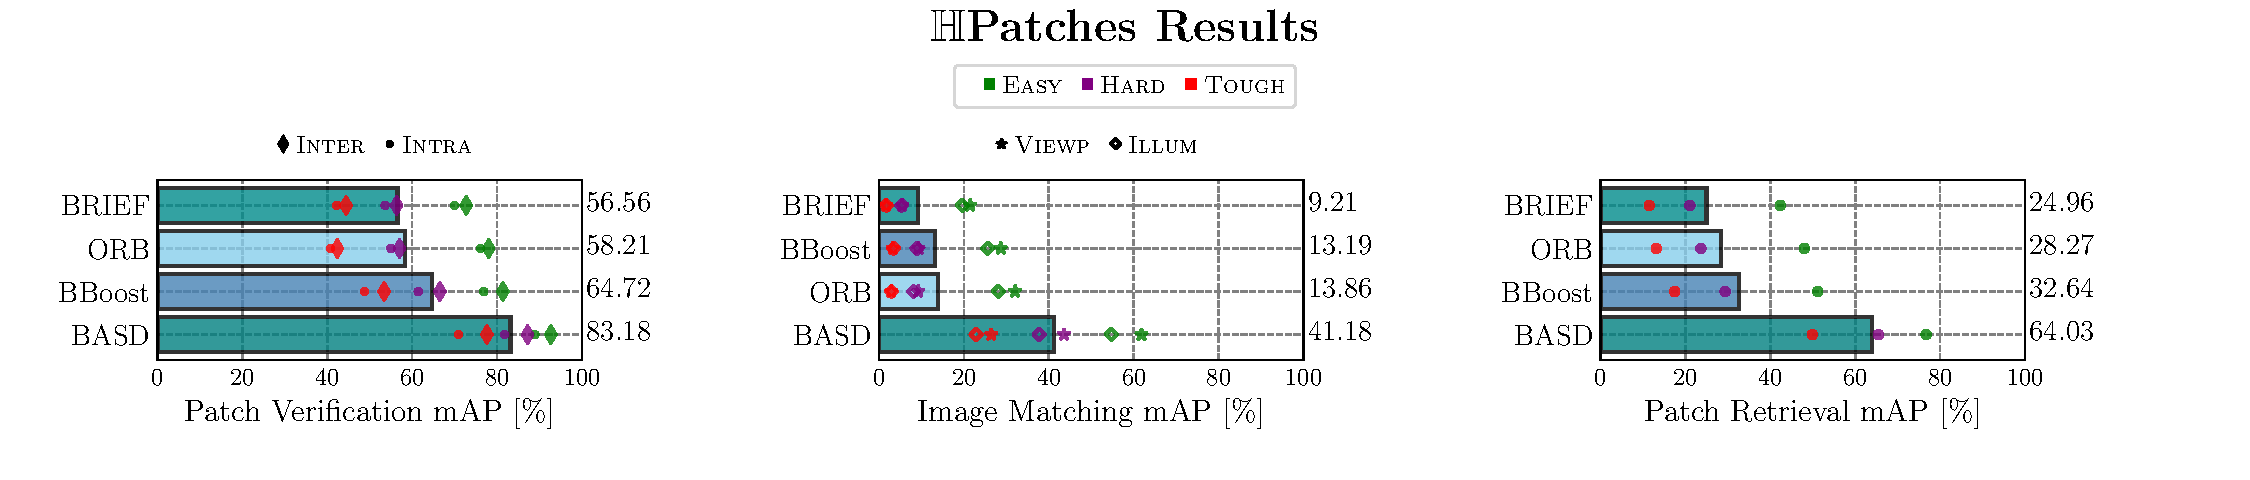
\includegraphics[scale=0.33]{HPatches--orb_brief_binboost_BASD}
\captionsetup{font={scriptsize}}
\caption{The HPatches Results.} \scriptsize
\end{figure}


\subsection{SLAM system evaluation}


\subsubsection{Evaluation of Tartanair dataset}
To evaluate the accuracy and robustness of our learned descriptor in BASD-SLAM, we introduce the Tartanair dataset \cite{c31} for localization  evaluation. Tartanair dataset is a new benchmark dataset collected in simulation,which can access precise ground truth labels. It contains multi-modal seneor data like RGB images,depth ,LiDAR data and so on. We compared our system with ORB-SLAM2, including the evaluation standard, ATE( absolute trajectory error) and SR(success rate). In order to present the robustness of our descriptor, we respectively chose two contexts in Tartanair, Japanese-Alley, and Ocean.Every single scene was runned five times,and chose output with the longest tracking time to compare with groundtruth.
The evaluation results are shown in TABLE I. The bold represents the better result. From the evaluation results above, we can easily draw the conclusion that our learned descriptor SLAM system outperforms the traditional descriptor SLAM system ORB-SLAM2.


%%%%%%%%%%%%%%%%%%%%%%%%%%%%%%%%%%%%%%%%%%%%%%table

\begin{table}[h]
\centering
\scriptsize
\caption{Comparison of SLAM performance with ORB and BASD descriptors . The BOLD Implies The Best Performace.}
\label{table_example}
\begin{center}
\begin{tabular}{ccccccc}
\toprule
\midrule
%%%%%
\multirow{2}{*}{Env Name} & \multirow{2}{*}{Sequence}  &\multirow{2}{*}{Motion Pattern} & \multicolumn{2}{c}{ORB} & \multicolumn{2}{c}{BASD}     \\%换行
  \cline{4-7}% 在3-8行绘制横线 
                                                      & \multicolumn{1}{c}{} & \multicolumn{1}{c}{}    & \multicolumn{1}{c}{ATE} & \multicolumn{1}{c}{SR} & \multicolumn{1}{c}{ATE}  & \multicolumn{1}{c}{SR}\\
  \cline{1-7}

%%%%%%%%%%%%%%%%%%%%%%%%%%%%%%%%%%%%%%%%%%%
\multirow{8}{*}{Japanese-alley}   &  \multirow{2}{*}{1}   &  \multicolumn{1}{c}{Easy}  & \multicolumn{1}{c}{1.639} & \multicolumn{1}{c}{0.999} & \multicolumn{1}{c}{\textbf{0.2214}}  & \multicolumn{1}{c}{\textbf{0.9999}}   \\
  \cline{3-7}

%%%%%%%
                                                         & \multicolumn{1}{c}{}  &  \multicolumn{1}{c}{Hard}  & \multicolumn{1}{c}{0.094} & \multicolumn{1}{c}{0.36196} & \multicolumn{1}{c}{\textbf{0.04127} } & \multicolumn{1}{c}{\textbf{0.3926}}   \\
  \cline{2-7}

%%%%%%%
                                   &  \multirow{2}{*}{2}   &  \multicolumn{1}{c}{Easy}  & \multicolumn{1}{c}{3.022} & \multicolumn{1}{c}{0.997} & \multicolumn{1}{c}{\textbf{0.2545}}  & \multicolumn{1}{c}{\textbf{1}}   \\
  \cline{3-7}
%%%%%%%
                                                          & \multicolumn{1}{c}{} &  \multicolumn{1}{c}{Hard}  & \multicolumn{1}{c}{0.8455} & \multicolumn{1}{c}{0.9949} & \multicolumn{1}{c}{\textbf{0.06}}  & \multicolumn{1}{c}{\textbf{0.9974}}   \\
  \cline{2-7}
                                    &  \multirow{2}{*}{3}   &  \multicolumn{1}{c}{Easy}  & \multicolumn{1}{c}{\textbf{0.0365}} & \multicolumn{1}{c}{0.133} & \multicolumn{1}{c}{0.30347}  & \multicolumn{1}{c}{\textbf{0.9928}}   \\
  \cline{3-7}
                                                          & \multicolumn{1}{c}{} &  \multicolumn{1}{c}{Hard}  & \multicolumn{1}{c}{1.672} & \multicolumn{1}{c}{\textbf{1}} & \multicolumn{1}{c}{\textbf{0.07559}}  & \multicolumn{1}{c}{0.9935}   \\
  \cline{2-7}
                                    &  \multirow{2}{*}{4}   &  \multicolumn{1}{c}{Easy}  & \multicolumn{1}{c}{0.0662} & \multicolumn{1}{c}{0.9897} & \multicolumn{1}{c}{\textbf{0.0356}}  & \multicolumn{1}{c}{\textbf{0.9987}}   \\
  \cline{3-7}
                                                          & \multicolumn{1}{c}{} &  \multicolumn{1}{c}{Hard}  & \multicolumn{1}{c}{0.155} & \multicolumn{1}{c}{1} & \multicolumn{1}{c}{\textbf{0.07665}}  & \multicolumn{1}{c}{1}   \\
 \cline{1-7}
%%%%%%%%%%%%%%%%%%%%%%%%%%%%%%%%%%%%%%%%%%%%%%%%%%%%%%%%%%%%%%%%

%%%%%%%%%%%%%%%%%%%%%%%%%%%%%%%%%%%%%%%%%%%
\multirow{8}{*}{Ocean}   &  \multirow{2}{*}{0}   &  \multicolumn{1}{c}{Easy}  & \multicolumn{1}{c}{0.8996} & \multicolumn{1}{c}{0.3179} & \multicolumn{1}{c}{\textbf{0.13248}}  & \multicolumn{1}{c}{\textbf{0.33}  } \\
  \cline{3-7}

%%%%%%%
                                                         & \multicolumn{1}{c}{}  &  \multicolumn{1}{c}{Hard}  & \multicolumn{1}{c}{\textbf{0.11326}} & \multicolumn{1}{c}{0.2861} & \multicolumn{1}{c}{0.7086}  & \multicolumn{1}{c}{\textbf{0.3514}}   \\
  \cline{2-7}

%%%%%%%
                                   &  \multirow{2}{*}{1}   &  \multicolumn{1}{c}{Easy}  & \multicolumn{1}{c}{0.3717} & \multicolumn{1}{c}{0.9081} & \multicolumn{1}{c}{\textbf{0.2922}}  & \multicolumn{1}{c}{\textbf{1}}   \\
  \cline{3-7}
%%%%%%%
                                                          & \multicolumn{1}{c}{} &  \multicolumn{1}{c}{Hard}  & \multicolumn{1}{c}{0.68} & \multicolumn{1}{c}{0.348} & \multicolumn{1}{c}{\textbf{0.0497}}  & \multicolumn{1}{c}{\textbf{0.36154}}   \\
  \cline{2-7}
                                    &  \multirow{2}{*}{2}   &  \multicolumn{1}{c}{Easy}  & \multicolumn{1}{c}{0.7493} & \multicolumn{1}{c}{0.9962} & \multicolumn{1}{c}{\textbf{0.3589}}  & \multicolumn{1}{c}{\textbf{0.998}}   \\
  \cline{3-7}
                                                          & \multicolumn{1}{c}{} &  \multicolumn{1}{c}{Hard}  & \multicolumn{1}{c}{5.292} & \multicolumn{1}{c}{0.78628} & \multicolumn{1}{c}{\textbf{2.7097}}  & \multicolumn{1}{c}{\textbf{0.7863}}   \\
  \cline{2-7}
                                    &  \multirow{2}{*}{4}   &  \multicolumn{1}{c}{Easy}  & \multicolumn{1}{c}{\textbf{0.05}} & \multicolumn{1}{c}{0.389} & \multicolumn{1}{c}{0.4442}  & \multicolumn{1}{c}{\textbf{0.5459}}   \\
  \cline{3-7}
                                                          & \multicolumn{1}{c}{} &  \multicolumn{1}{c}{Hard}  & \multicolumn{1}{c}{0.1457} & \multicolumn{1}{c}{0.9979} & \multicolumn{1}{c}{\textbf{0.1066}}  & \multicolumn{1}{c}{\textbf{0.9979}}   \\
%%%%%%%%%%%%%%%%%%%%%%%%%%%%%%%%%%%%%%%%%%%%%%%%%%%%%%%%%%%%%%%%

\midrule
\toprule
\end{tabular} 
\end{center}
\end{table}
\vspace{-0.47cm}

%%%%%%%%%%%%%%%%%%%%%%%%%%%%%%%%%%%%%%%%%%%%%%%%%%%%%%%%%%%%%%%%%%%%%%%%%%%%%%

\section{CONCLUSIONS}

In this paper, we have presented a novel binary learning descriptor,which binarized ASD descriptor , and got more efficient and acuurate descriptor. Our binary method takes even-distribution ,correlation and quantization loss, which can be trained very easily. The output showed that our descriptor outperformed traditinal binary descriptor. We also present a SLAM system with our learning descriptor , And it also has outstanding advantages than traditional ORB descriptor in complex secenarios in Tartanair dataset.


%%%%%%%%%%%%%%%%%%%%%%%%%%%%%%%%%%%%%%%%%%%%%%%%%%%%%%%%%%%%%%%%%%%%%%%%%%%%%%
\section*{ACKNOWLEDGMENT}

This work is supported by The National Key Research and Development Program of China under Project of 2017YFB0102503 and the National Natural Science Foundation of China under Project of 51605285.



%%%%%%%%%%%%%%%%%%%%%%%%%%%%%%%%%%%%%%%%%%%%%%%%%%%%%%%%%%%%%%%%%%%%%%%%%%%%%%%%

\begin{thebibliography}{99}




%%%%introduction leave 5 articles

%%%%%%%%%%%%%%%%%%%%%%%%%%%%%%%




\bibitem{c1} Lowe D G . Distinctive Image Features from Scale-Invariant Keypoints[J]. International Journal of Computer Vision, 2004, 60(2):91-110.
\bibitem{c2} Bay H , Ess A , Tuytelaars T , et al. Speeded-Up Robust Features (SURF)[J]. Computer Vision and Image Understanding, 2008, 110(3):346-359.
\bibitem{c3} Rublee E , Rabaud V , Konolige K , et al. ORB: An efficient alternative to SIFT or SURF[C]// 2011 International Conference on Computer Vision. IEEE, 2012.
\bibitem{c4} Mur-Artal R , Montiel J M M , Tardos J D . ORB-SLAM: a Versatile and Accurate Monocular SLAM System[J]. IEEE Transactions on Robotics, 2015, 31(5):1147-1163.
\bibitem{c5} Simo-Serra E , Trulls E , Ferraz L , et al. Discriminative Learning of Deep Convolutional Feature Point Descriptors[C]// 2015 IEEE International Conference on Computer Vision (ICCV). IEEE, 2016.
%%%%%%%%%%%%%%%%%%%%%%%%%


\bibitem{c6} Lowe D G . Distinctive Image Features from Scale-Invariant Keypoints[J]. International Journal of Computer Vision, 2004, 60(2):91-110.
\bibitem{c7} K  Daniilidis,  Maragos P ,  Paragios N . [Lecture Notes in Computer Science] Computer Vision – ECCV 2010 Volume 6314 || BRIEF: Binary Robust Independent Elementary Features[J].  2010, 10.1007/978-3-642-15561-1(Chapter 56):778-792.
\bibitem{c8} Rublee E ,  Rabaud V ,  Konolige K , et al. ORB: an efficient alternative to SIFT or SURF[C]// IEEE International Conference on Computer Vision, ICCV 2011, Barcelona, Spain, November 6-13, 2011. IEEE, 2011.
\bibitem{c9} Ke N Y ,  Sukthankar R . PCA-SIFT: a more distinctive representation for local image descriptors[C]// IEEE Computer Society Conference on Computer Vision  Pattern Recognition. IEEE Computer Society, 2004.
\bibitem{c10} T. Trzcinski, M. Christoudias, P. Fua, and V. Lepetit. Boosting binary keypoint descriptors. In Proceedings of the IEEE conference on computer vision and pattern recognition, pages 2874–2881, 2013.
\bibitem{c11} Y. Gao, W. Huang and Y. Qiao, ”Local Multi-Grouped Binary Descriptor With Ring-Based Pooling Configuration and Optimization,” in IEEE Transactions on Image Processing, vol. 24, no. 12, pp. 4820-4833, Dec. 2015.
\bibitem{c12} D. DeTone, T. Malisiewicz and A. Rabinovich, ”SuperPoint: SelfSupervised Interest Point Detection and Description,” 2018 IEEE/CVF Conference on Computer Vision and Pattern Recognition Workshops (CVPRW), Salt Lake City, UT, 2018, pp. 337-33712.
\bibitem{c13} Han X ,  Leung T ,  Jia Y , et al. MatchNet: Unifying feature and metric learning for patch-based matching[C]// Computer Vision  Pattern Recognition. IEEE, 2015.
\bibitem{c14} Tian Y ,  Fan B ,  Wu F . L2-Net: Deep Learning of Discriminative Patch Descriptor in Euclidean Space[C]// 2017 IEEE Conference on Computer Vision and Pattern Recognition (CVPR). IEEE, 2017.
\bibitem{c15} A. Mishchuk, D. Mishkin, F. Radenovic, and J. Matas, “Working hard to know your neighbor’s margins: Local descriptor learning loss,” in Advances in Neural Information Processing Systems, 2017, pp. 4826–4837.

\bibitem{c16} Duan Y ,  Lu J ,  Wang Z , et al. Learning Deep Binary Descriptor with Multi-quantization[C]// Computer Vision and Pattern Recognition. IEEE, 2017.
\bibitem{c17} Do T T ,  Doan A D ,  Cheung N M . Learning to Hash with Binary Deep Neural Network[J]. Springer, Cham, 2016.
\bibitem{c18} Ye J ,  Zhang S ,  Huang T , et al. CDbin: Compact Discriminative Binary Descriptor Learned with Effcient Neural Network[J]. IEEE Transactions on Circuits and Systems for Video Technology, 2019:1-1.
\bibitem{c19} Wang S ,  Clark R ,  Wen H , et al. DeepVO: Towards end-to-end visual odometry with deep Recurrent Convolutional Neural Networks[C]// 2017 IEEE International Conference on Robotics and Automation (ICRA). IEEE, 2017.
\bibitem{c20} Zhou T ,  Brown M ,  Snavely N , et al. Unsupervised Learning of Depth and Ego-Motion from Video[C]// 2017 IEEE Conference on Computer Vision and Pattern Recognition (CVPR). IEEE, 2017.
\bibitem{c21} Ummenhofer B ,  Zhou H ,  Uhrig J , et al. DeMoN: Depth and Motion Network for Learning Monocular Stereo[C]// 2017 IEEE Conference on Computer Vision and Pattern Recognition (CVPR). IEEE, 2017.
\bibitem{c22} Salas-Moreno R F ,  Newcombe R A ,  Strasdat H , et al. SLAM++: Simultaneous Localisation and Mapping at the Level of Objects[C]// Computer Vision and Pattern Recognition. IEEE, 2013.
\bibitem{c23} Stenborg E ,  Toft C ,  Hammarstrand L . Long-term Visual Localization using Semantically Segmented Images[C]// 2018:6484-6490.
\bibitem{c24} Li J ,  Koreitem K ,  D  Meger, et al. View-Invariant Loop Closure with Oriented Semantic Landmarks[C]// 2020 IEEE International Conference on Robotics and Automation (ICRA). IEEE, 2020.
\bibitem{c25} Mur-Artal R ,  Montiel J M M ,  Tardos J D . ORB-SLAM: A Versatile and Accurate Monocular SLAM System[J]. IEEE Transactions on Robotics, 2015, 31(5):1147-1163.
\bibitem{c26}
\bibitem{c27}
\bibitem{c28} Ma T ,  Y  Wang,  Wang Z , et al. ASD-SLAM: A Novel Adaptive-Scale Descriptor Learning for Visual SLAM[C]// 2020 IEEE Intelligent Vehicles Symposium (IV). IEEE, 2020.
\bibitem{c29} S. Winder and M. Brown. Learning Local Image Descriptors. To appear International Conference on Computer Vision and Pattern Recognition (CVPR2007)
\bibitem{c30} Balntas V ,  Lenc K ,  Vedaldi A , et al. HPatches: A Benchmark and Evaluation of Handcrafted and Learned Local Descriptors[C]// IEEE Conference on Computer Vision and Pattern Recognition. IEEE Computer Society, 2017.
\bibitem{c31} Wang W ,  Zhu D ,  Wang X , et al. TartanAir: A Dataset to Push the Limits of Visual SLAM[J]. arXiv, 2020.

\end{thebibliography}







\vspace{12pt}
\color{red}
IEEE conference templates contain guidance text for composing and formatting conference papers. Please ensure that all template text is removed from your conference paper prior to submission to the conference. Failure to remove the template text from your paper may result in your paper not being published.

\end{document}
